\chapter{Анализ методов и технологий обработки рукописного наследия}
\label{chapter1}

\section{Анализ достоинств и недостатков алгоритмов и программных средств сегментации и классификации крюков и знамён, разработанных для Корпуса рукописного наследия Древней Руси}

\subsection{Средства сегментации крюков и знамен портала}

Для сегментации областей, которые потом будут классифицироваться, применяется алгоритм MSER.

\textbf{Алгоритм MSER (Maximally Stable Extremal Regions)} был предложен Матушем Матейкой и 
Джереми М. Максаном в 2002 году. Этот метод был разработан для выделения стабильных 
областей на изображении, которые остаются неизменными в широком диапазоне пороговых значений. 
MSER нашел широкое применение в задачах компьютерного зрения, таких как распознавание объектов, 
отслеживание и сегментация изображений\cite{MGonsales}.


Алгоритм состоит из следующих этапов:

\textit{Пороговая сегментация} — Изображение многократно сегментируется при различных порогах. Для каждого порога определяются связные компоненты. 
		Связанная компонента — это множество пикселей, которые соединены друг с другом и имеют одинаковое значение интенсивности. \\
		Формула для пороговой сегментации:
		\begin{center}
			$I_T(x, y) = 
			\begin{cases} 
			1 & \text{если } I(x, y) \ge T \\
			0 & \text{если } I(x, y) < T 
			\end{cases}$,
		\end{center}

\textit{Экстремальные области} — связные компоненты, которые либо полностью темнее (темная область на светлом фоне), 
		либо полностью светлее (светлая область на темном фоне), чем ее окружение. \\
		Связанная компонента \( C \) при пороге \( T \) считается экстремальной областью, если:
		\begin{center}
			$\forall (x, y) \in C \quad \forall (x', y') \in \partial C \quad I(x, y) < I(x', y')$
		\end{center}
		где \( \partial C \) — граница области \( C \).

\textit{Стабильность области} —  определяется по изменению ее размера при изменении порога. 
		Область считается максимально стабильной, если изменение ее размера минимально при изменении порога. \\
		Формула для определения стабильности области:
		\begin{center}
			$\Delta(C) = \frac{|C_{T+\Delta T}| - |C_T|}{\Delta T}$
		\end{center}
		где \(|C_T|\) — размер компоненты \(C\) при пороге \(T\).
\textit{Выбор максимальных стабильных областей} \\
		Области, которые остаются стабильными в широком диапазоне порогов, выбираются в качестве конечных регионов.

Преимущества и недостатки MSER\cite{MPrinse}

\textit{Преимущества}
	\begin{itemize}
		\item Независимость от масштаба: MSER эффективно выделяет области при изменении масштаба изображения.
		\item Робастность к освещению: Метод хорошо работает в условиях изменяющегося освещения.
		\item Высокая производительность: MSER работает быстро и эффективно для многих приложений.
	\end{itemize}


\textit{Недостатки}
	\begin{itemize}
		\item Чувствительность к шуму: Алгоритм может выделять ложные области в присутствии значительного шума.
		\item Проблемы с текстурированными фонами: На текстурированных изображениях может выделяться много ненужных областей.
	\end{itemize}



\subsection{Средства классификации крюков и знамен портала}

После сегментации изображения на устойчивые области, по каждой выделенной 
области собираются следующие признаки:



		\textit{Моменты изображения} — это количественные характеристики, 
		которые описывают распределение пикселей в области. Они могут использоваться 
		для вычисления различных свойств объекта, таких как площадь, центр тяжести и 
		инерционные характеристики. Моменты до второго порядка часто используются для 
		описания базовых свойств изображения\cite{MGonsales}. \\
		Формула для вычисления геометрических моментов \( m_{pq} \):
		\begin{center}
			$m_{pq} = \sum_{x}\sum_{y} x^p y^q I(x, y)$
		\end{center}
		где \( I(x, y) \) — интенсивность пикселя в точке \((x, y)\).
		Используются для:
		\begin{itemize}
			\item Оценки площади объекта.
			\item Нахождения центра масс объекта.
			\item Вычисления инерционных характеристик.
		\end{itemize}

		\textit{Hu моменты} — это набор из 7 чисел, которые вычисляются с использованием 
		центральных моментов и являются инвариантными к преобразованиям изображения.
		Первые 6 моментов инвариантны к переводу, масштабированию, вращению и отражению. 
		При этом знак 7-го момента меняется при отражении изображения\cite{MIsyacan}.
		\begin{center}
			$\phi_1 = \eta_{20} + \eta_{02}$ \\
			$\phi_2 = (\eta_{20} - \eta_{02})^2 + 4\eta_{11}^2$ \\
			$\phi_3 = (\eta_{30} - 3\eta_{12})^2 + (3\eta_{21} - \eta_{03})^2$ \\
			$\phi_4 = (\eta_{30} + \eta_{12})^2 + (\eta_{21} + \eta_{03})^2$ \\
			$\phi_5 = (\eta_{30} - 3\eta_{12})(\eta_{30} + \eta_{12})(\eta_{30} + \eta_{12})^2 - 3(\eta_{21} + \eta_{03})^2$ \\
			$\phi_6 = (\eta_{20} - \eta_{02})[(\eta_{30} + \eta_{12})^2 - (\eta_{21} + \eta_{03})^2]\quad + 4\eta_{11}(\eta_{30} + \eta_{12})(\eta_{21} + \eta_{03})$ \\
			$\phi_7 = (3\eta_{21} - \eta_{03})(\eta_{30} + \eta_{12})[(\eta_{30} + \eta_{12})^2 - 3(\eta_{21} + \eta_{03})^2]\quad - (\eta_{30} - 3\eta_{12})(\eta_{21} + \eta_{03})[3(\eta_{30} + \eta_{12})^2 - (\eta_{21} + \eta_{03})^2]$
		\end{center}
\textit{Профили изображения\cite{MSofier}}
		\begin{itemize}
			\item Вертикальный профиль: сумма пикселей в каждом ряду изображения. 
				Он помогает понять вертикальное распределение интенсивности пикселей в изображении. \\
				\begin{center}
					$V(y) = \sum_{x} I(x, y)$
				\end{center}
				где \( V(y) \) — значение вертикального профиля на \( y \)-й строке, 
				\( I(x, y) \) — интенсивность пикселя в точке \((x, y)\).
			\item Горизонтальный профиль: сумма пикселей в каждом столбце изображения. 
				Он помогает понять горизонтальное распределение интенсивности пикселей в изображении. \\
				\begin{center}
					$H(x) = \sum_{y} I(x, y)$
				\end{center}
				где \( H(x) \) — значение горизонтального профиля на \( x \)-й колонке, 
				\( I(x, y) \) — интенсивность пикселя в точке \((x, y)\).
		\end{itemize}

		\textit{Фурье-дескрипторы} — это коэффициенты преобразования Фурье, которые используются 
		для описания формы контура объекта. Они позволяют сравнивать формы объектов, 
		независимо от их положения, масштаба и ориентации\cite{MShtepa}. \\

		Процесс вычисления Фурье-дескрипторов включает следующие шаги:
		\begin{itemize}
			\item Представление контура объекта в виде комплексной функции.
			\item Применение быстрого преобразования Фурье.
			\item Нормализация дескрипторов для обеспечения инвариантности к масштабу, вращению и сдвигу.
		\end{itemize}
		Формула для вычисления дескрипторов Фурье:
		\begin{center}
			$S(k) = \sum_{n=0}^{N-1} s(n) e^{-i \frac{2 \pi k n}{N}}$
		\end{center}
		где \( S(k) \) — \( k \)-й дескриптор Фурье, \( s(n) \) — координата \( n \)-й точки контура, \( N \) — общее количество точек на контуре.


\textit{Площадь символа}
		Вычисляется через момент:
		\begin{center}
			$\text{area} = m_{00}$
		\end{center}


\textit{Центр тяжести} — точка, представляющая собой 
		среднее положение всех пикселей в объекте. Он характеризует положение 
		объекта в пространстве изображения и используется для описания и анализа 
		форм объектов, их отслеживания и выравнивания\cite{MGladkikh}.
		\begin{center}
			$x_c = \frac{m_{10}}{m_{00}}, \quad y_c = \frac{m_{01}}{m_{00}}$
		\end{center}


\textit{Ориентация} — угол, под которым ориентирован объект относительно осей
		координат. Вычисляется из ковариационной матрицы:
		\begin{center}
			$\text{angle} = \frac{1}{2} \arctan\left(\frac{2 \cdot \text{cov}(x, y)}{\text{var}(x) - \text{var}(y)}\right)$
		\end{center}
		где \( \text{cov}(x, y) \) — ковариация координат \( x \) и \( y \), \( \text{var}(x) \) и \( \text{var}(y) \) — дисперсии координат \( x \) и \( y \).


		\textit{Эксцентриситет} — мера отклонения формы объекта от круга. 
		Вычисляется из ковариационной матрицы:
		\begin{center}
			$\text{eccentricity} = \sqrt{1 - \frac{\lambda_2}{\lambda_1}}$
		\end{center}
		где \( \lambda_1 \) и \( \lambda_2 \) — собственные значения ковариационной матрицы.


		\textit{Рациональность формы} — это отношение площади к квадрату периметра объекта\cite{MYarovoy}.
		\begin{center}
			$Rc = \frac{4 \pi \cdot \text{area}}{\text{perimeter}^2}$
		\end{center}
		где \( \text{area} \) — площадь объекта, \( \text{perimeter} \) — периметр объекта.


\textit{Отношение максимального диаметра к периметру}
		\begin{center}
			$D/P = \frac{\text{max\_diameter}}{\text{perimeter}}$
		\end{center}


После обработки всех сегментов, для каждого сегмента мы получаем вектор признаков. 
Далее, перед тем как использовать эти признаки для классификации, мы применяем метод
робастого масштабирования для нормализации данных.

Метод масштабирует признаки так, чтобы медиана каждого признака была равна нулю, 
а интерквартильный размах (разница между 75-м и 25-м процентилями) — равен единице\cite{MJHan}. 

Для каждого признака \( x \) рассчитываем медиану \( Q_2 \) и интерквартильный размах 
\( IQR = Q_3 - Q_1 \), где \( Q_1 \) — это 25-й перцентиль, а \( Q_3 \) — это 75-й перцентиль. 
Преобразованный признак \( x' \) вычисляется как:

\begin{center}
	$x' = \frac{x - Q_2}{IQR}$
\end{center}
  
После масштабирования признаков сегментов, мы применяем логистическую регрессию для 
определения класса сегмента.

Логистическая регрессия — это метод машинного обучения, который используется для 
решения задач бинарной классификации. Целью логистической регрессии является предсказание 
вероятности принадлежности объекта к одному из двух классов на основе одного или 
нескольких (признаков). Основным компонентом логистической регрессии является 
логистическая функция (сигмоида), которая преобразует линейную комбинацию 
признаков в вероятность\cite{MSergeev}:

\begin{center}
	$P(y=1|X) = \frac{1}{1 + e^{-(\beta_0 + \beta_1 X_1 + \cdots + \beta_n X_n)}}$
\end{center}

где \( P(y=1|X) \) — вероятность принадлежности к классу 1, \( \beta_0, \beta_1, \ldots, \beta_n \) — параметры модели (веса), и \( X_1, \ldots, X_n \) — входные признаки.

Для определения весов логистической регрессии, мы подготовили обучающую выборку, состоящую из 100 
аннотированных лингвистами страниц рукописей. Каждая страница была вручную сегментирована и 
классифицирована, что позволяет нам знать точный класс каждого сегмента. Модель логистической регрессии 
обучена таким образом, чтобы при сочетании весов с признаками сегмента вероятность правильной классификации 
была максимальной.

Для наших сегментированных областей, мы поступаем следующим образом:
Для каждого класса модель логистической регрессии вычисляет вероятность принадлежности сегмента 
к этому классу. Затем для классификации сегмента мы выбираем класс с наибольшей вероятностью.

Подведем итоги сегментации представленной в Корпусе


\textit{Достоинства}
	\begin{itemize}
		\item Устойчивость к выбросам: Использование масштабирования признаков делает модель менее чувствительной к выбросам, 
			что повышает общую надежность и устойчивость классификации\cite{MIvaschenko}.
		\item Относительно высокая точность, если классифицируемая рукопись похожа на обучающую выборку
	\end{itemize}


\textit{Недостатки}
	\begin{itemize}
		\item Чувствительность к мультиколлинеарности: Модель логистической регрессии может быть 
			чувствительна к сильной корреляции между признаками, что может ухудшить её способность 
			к обобщению на новых данных\cite{MKurdyumov}.
		\item Ограниченная адаптация: Модель, обученная на одном наборе данных, может плохо адаптироваться 
			к другим наборам данных, которые могут отличаться по качеству или характеру сегментов, 
			требуя дополнительного обучения или доработки.
		\item Проблемы с редкими классами: Логистическая регрессия может плохо работать с очень редкими 
			классами, так как данные для этих классов могут быть недостаточно репрезентативными, 
			что приводит к плохой классификации таких сегментов.
		\item Проблемы с масштабируемостью: Хотя логистическая регрессия быстро обучается на небольших 
			наборах данных, на очень больших и сложных наборах данных процесс обучения и предсказания 
			может стать ресурсоемким и менее эффективным.
	\end{itemize}


\begin{figure}[h]
	\begin{center}
		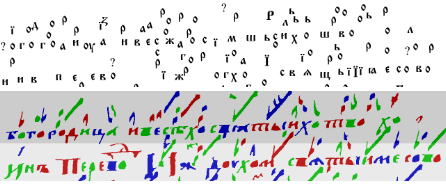
\includegraphics[width=.5\columnwidth]{./img/wrongClassification+Segment.png}%
	\end{center}
	\caption{Пример классификации крюков, при отсутствии их в обучающей модели. Снизу — сегментированные участки, сверху — их классификация.}%
	\label{pic:wrongClassificator}%
\end{figure}

\section{Исследование правил позиционирования крюков и знамён над словами в текстах рукописей}

Крюки и знамена — знаки русского старинного безлинейного нотного письма.
Применялись в Русской Православной Церкви в XI—XVIII вв. Название получили от одного
из наиболее употребительных знаков этой системы — «крюка». Число крюков превышало 70, каждый 
из них обозначал от одного до нескольких звуков различной высоты и длительности. Пение по крюкам называлось 
крюковым, или знаменным пением\cite{MKazantsev}.

%%% здесь все из книги григорьева

Согласно \cite{MGrigoriev}, разнообразие знамен графически образуется из небольшого числа основных элементарных 
знамен.
\begin{figure}[H]
	\begin{center}
		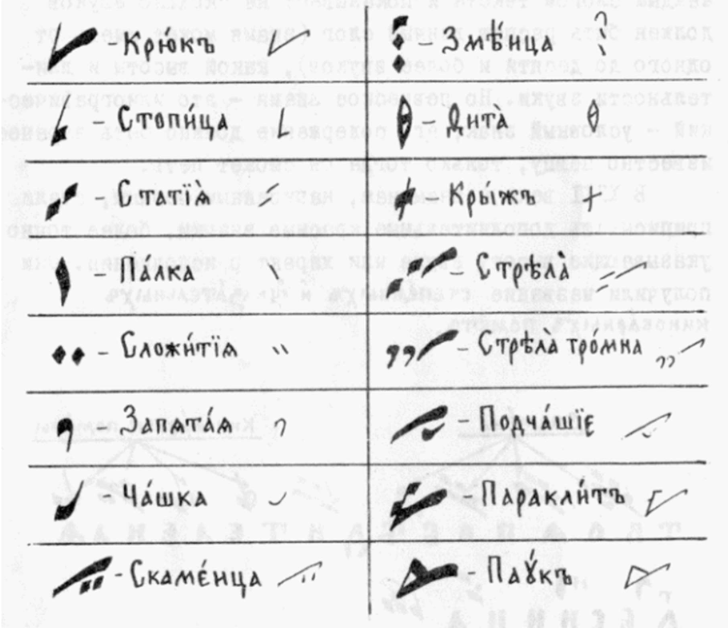
\includegraphics[width=.5\columnwidth]{./img/hooks_base.png}%
	\end{center}
	\caption{Начертания простых знамен.}%
	\label{pic:hooks_base}%
\end{figure}

Из начертаний отдельных знамен образуются целые сочетания, например.
\begin{figure}[H]
	\begin{center}
		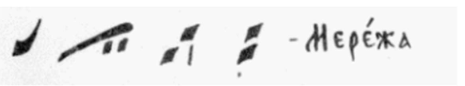
\includegraphics[width=.5\columnwidth]{./img/hooks_mod_base.png}%
	\end{center}
	\caption{Пример сочетания знамен.}%
	\label{pic:hooks_mod_base}%
\end{figure}


В основном у часто используемых крюков, встречаются 3 версии: простая, мрачная, и светлая
\begin{figure}[H]
	\begin{center}
		
\includegraphics[width=.5\columnwidth]{./img/strels_mods.png}%
	\end{center}
	\caption{Основная разновидность стрел.}%
	\label{pic:strels_mods}%
\end{figure}


\begin{figure}[H]
	\begin{center}
		
\includegraphics[width=.5\columnwidth]{./img/dots_mods.png}%
	\end{center}
	\caption{Основная разновидность статьи.}%
	\label{pic:dots_mods}%
\end{figure}


Опираясь на общие и усреднённые знания о крюках и знаменах, можно выделить несколько основных правил их 
позиционирования\cite{MGrigoriev}:

\begin{itemize}
	\item Стопица (см. рис. \ref{pic:allhooksdesc}): Ставится на слогах, не имеющих ударения, или там, где напев движется звуками одинаковой высоты, рецитативом. 
		Эти звуки не сильные, напоминают простой мерный шаг.
	
	\item Запятая (см. рис. \ref{pic:allhooksdesc}): Понижает высоту в напеве или указывает низкий звук, от которого напев устремляется вверх. Звук большей силы, чем у стопицы. 
		Преимущественно ставится над гласными.

	\item Крюк (см. рис. \ref{pic:allhooksdesc}): Знамя крюка повышает высоту в напеве. Ставится на ударных слогах или слогах, наиболее важных по смыслу. 
		В зависимости от значимости слога или высоты звука, крюк бывает простым, луночным и т. д. Обеспечивает полное, 
		сильное и яркое звучание.

	\item Параклит (см. рис. \ref{pic:allhooksdesc}): Ставится в начале слова или предложения, в котором содержится обращение к Богу, святым, часто в 
		начале песнопения. Указывает на необходимость внимания и благоговения. На низких звуках обычно не используется. 
		Звучит сходно с крюком простым.
	
	\item Статьи (см. рис. \ref{pic:allhooksdesc}): Ставится чаще в конце попевок или на ударных слогах. В зависимости от значения звука или его высоты, 
		как и крюки, бывает простым, луночным и светлым. Обеспечивает полное, сильное и яркое звучание, длительность 
		несколько больше обычной.
\end{itemize}

\begin{figure}[H]
	\begin{center}
		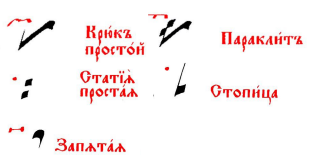
\includegraphics[width=.5\columnwidth]{./img/hooks/allhooksdesc.png}%
	\end{center}
	\caption{Основные крюки.}%
	\label{pic:allhooksdesc}%
\end{figure}

Во времена Древней Руси уровень грамотности был низким, и писари, занимавшиеся крюковой нотацией, часто опирались на свои локальные 
традиции и навыки. Хотя существовало общее понимание использования крюков, точных правил их позиционирования 
не было. Каждый писарь мог вносить свои индивидуальные особенности в запись крюков, что приводило к значительным 
региональным различиям. Это объясняет, почему в разных рукописях встречаются уникальные крюки и варианты их 
расположения, не описанные в известных букварях\cite{MShulgin}.

Крюки использовались для распевки, поэтому их расположение над гласными буквами было естественным, так как именно 
гласные формируют пение. Однако из приведённых примеров ясно, что многие крюки могут обозначать общий характер 
пропева перед слогом, поэтому они могут располагаться над согласными буквами, перед слогами, в начале или в конце
слова. Если идёт сложная и переливистая пропевка, крюки могут располагаться вне слов. Также не стоит забывать, что 
не все писари придерживались даже этих правил\cite{MShulgin}.

\begin{figure}[H]
	\begin{center}
		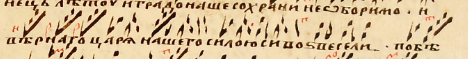
\includegraphics[width=.5\columnwidth]{./img/exampleReal.png}%
	\end{center}
	\caption{Пример старославянской рукописи XVII века.}%
	\label{pic:realexample}%
\end{figure}


\section{Анализ подходов к формированию и представлению обучающих выборок для нейросетевых моделей}

Для формирования первичной выборки нейросетевой модели были выбраны различные рукописи XVII века. 
Эти рукописи обычно обладают более высоким качеством, что позволяет создавать высококачественную обучающую 
выборку. Высококачественные данные упрощают процесс обучения нейросетевой модели, повышая её точность и 
эффективность.


После сбора данных необходимо выполнить предобработку, чтобы повысить их общее качество и подготовить к 
обучению модели. Существуют различные подходы к предобработке данных:

	\textit{Нормализация изображений}: Приведение всех изображений крюков к единой форме и размеру 
		(например, \(64 \times 64\) пикселей). Это упростит обработку данных и их представление в модели.
		Однако возможна потеря деталей из-за масштабирования.
		
	\textit{Улучшение качества изображений}: Фильтрация шума и улучшение контрастности изображений с 
		использованием различных алгоритмов фильтрации.

	\textit{Кодирование категориальных данныx}: Кодирование категориальных признаков (например, типов крюков) 
		в числовые значения с использованием методов, таких как one-hot encoding. Он подразумевает формирование
		бинарного вектора, где каждый столбей соответствует категории.

	\textit{Аугментация данных}: Для искусственного увеличения обучающей выборки используются методы аугментации данных.
		\begin{itemize}
			\item Геометрические преобразования: Применение преобразований, таких как вращение, сдвиг, масштабирование и отражение, к изображениям.
				Преобразования способствуют увеличению разнообразия данных и устойчивости модели к различным вариантам представления крюков.
			\item Цветовые преобразования: Изменение яркости, контраста и добавление цветового шума к изображениям. 
				Модель станет устойчивей к некачественным данным.
		\end{itemize}
	
	\textit{Балансировка данных}: Для устранения дисбаланса классов в данных используются следующие методы
		\begin{itemize}
			\item Oversampling: Увеличение числа данных меньшинств путём дублирования существующих примеров
			\item Undersampling: Уменьшение числа данных большинства путём удаления некоторых образцов.
		\end{itemize}
		Недостатком Oversampling является возможное переобучение на дублированных данных. Недостаток Undersampling
		в потеря части данных. Для нашего проекта приоритетом является кол-во данных, так как результирующие
		нотированные нейросетью рукописи будут постоянно просматриваться и изучаться лингвистами.
		\begin{itemize}
			\item SMOTE (Synthetic Minority Over-sampling Technique): Генерация новых образцов меньшинств путём 
				интерполяции между существующими данными.
		\end{itemize}

	\textit{Представление данных в виде тензоров}: 
		Каждое изображение крюка представляется в виде тензора размером \(1 \times 64 \times 64\) (для черно-белых изображений). 
		Тензорное представление позволяет эффективно обрабатывать изображения с использованием сверточных слоев. Тензорное представление
		данных позволяет удобно использовать сверточную нейросетью
	
	\textit{Сверточная нейронная сеть}:
		У данной разновидности нейронных сетей один из лучших
		алгоритмов распознавания и классификации изображений. По сравнению с полносвязной
		нейронной сетью у нее гораздо меньше количество настраиваемых весов.
		Главной особенностью свёрточной нейронной сети является «свертка». Процесс
		«свертки» представляет собой уменьшение размера матрицы признаков входного
		изображения\cite{MIvaschenko}.\\ 
		Для получения ячейки матрицы уменьшенного размера элементы исходной
		матрицы в определенной области умножают на вес с последующим суммированием всех
		элементов в этой области. Чтобы получить следующую ячейку уменьшенной матрицы
		происходит сдвиг области и выполнение тех же действий. Описанную выше
		последовательность действий можно записать формулой:
		\begin{center}
			$(I \times K)_{xy} = \sum_{i=1}^{h}\sum_{j=1}^{W} K_{ij} \times I_{x+i-1,y+k-1}$
		\end{center}
		где \( I \) — исходная матрица признака,  \( K \) матрица веса, \( x, y \) индексы выбранного блока,
		\( h, w \) — высота и ширина.
		\begin{figure}[H]
			\begin{center}
				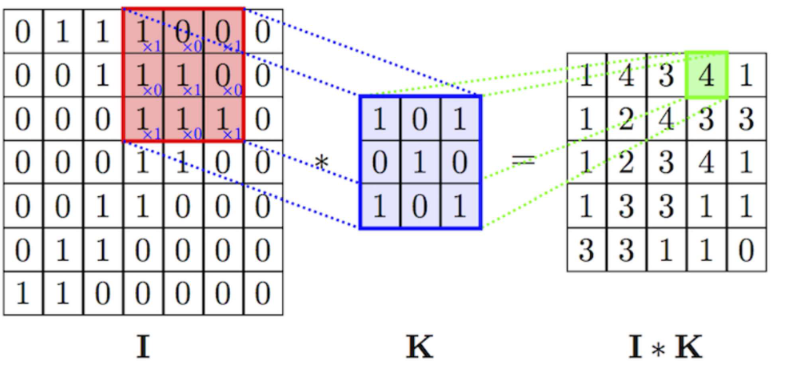
\includegraphics[width=.5\columnwidth]{./img/svertkaNeiro.png}%
			\end{center}
			\caption{Пример работы сверточной нейронной сети.}%
			\label{pic:svertkaNeiro}%
		\end{figure}

Подводя итоги методов и подходов формирования выборки, можно сделать вывод: Для нашей задачи 
наиболее подходящим методом является использование сверточных нейросетей, которые хорошо справляются 
с распознаванием и извлечением признаков из изображений. Основные аспекты нашей стратегии следующие:

\begin{itemize}
	\item Выборка собирается вручную из хорошо бинаризированных рукописей XVII века. Это позволяет обеспечить высокое качество исходных данных, что упрощает процесс обучения модели.
	\item Нормализация изображений проводится с использованием масок размером \(256 \times 256\) пикселей. Это обеспечивает единообразие и подходит для входных слоев нейросетей.
	\item Улучшение качества изображений (например, фильтрация шума или повышение контрастности) не требуется из-за высокой изначальной чёткости сканов.
	\item Категориальные данные кодируются сведениями о принадлежности крюка к определённому классу с использованием One-Hot Encoding или Label Encoding, что позволяет модели эффективно обучаться на этих данных.
	\item Основные геометрические преобразования включают масштабирование изображений до нужного размера. Повороты и отражения нецелесообразны в контексте крюков, так как они могут исказить их значение.
	\item Дополнительные методы аугментации включают наложение шумов и размытия. Это повышает устойчивость модели и её способность к общему распознаванию символов в различных условиях.
	\item Для сбалансированной работы модели важно, чтобы обучающая выборка была разнообразной и включала равное количество примеров различных крюков.
	\item Выбор сверточной нейросети обуславливает необходимость наличия большой и сбалансированной выборки. В нашем случае, для балансировки данных целесообразно использовать метод OverSampling.
\end{itemize}

\section{Выводы}

\begin{enumerate}
	\item Выполненный анализ средств классификации показывает их несостоятельность для крюков и знамен. Требуется
		улучшение модели классификации обновлением выборки или другой подход основанный на нейросетях.

	\item  Были исследованы правила позиционирования крюков в старославянских текстах. Часто встречаются локальные 
		и региональные особенности, что не позволяет выработать единую четкую картину. Отсутствие единого 
		стиля делает практически невозможной разработку обычного классификационного алгоритма связи букв и крюков.

	\item Проанализированы подходы к формированию и представлению выборок данных для обучения нейросетевых 
		моделей. Данный анализ позволяет выработать стратегию оптимального взаимодействия с собранными данными.
\end{enumerate}



\section{Постановка задачи учебно исследовательской работы}

В рамках разработки системы сегментации и классификации крюков и знамен в старославянских текстах 
выделяются следующие задачи:

\begin{itemize}
	\item Формирование выборки для нейросетевой модели распознавания крюков и знамен
	\item Модификация модели представления результатов сегментации страницы Корпуса, поддержка крюков и знамён 
	\item Интеграция средств сегментации и классификации крюков в портал
\end{itemize}

%%% Local Variables:
%%% TeX-engine: xetex
%%% eval: (setq-local TeX-master (concat "../" (seq-find (-cut string-match ".*-3-pz\.tex$" <>) (directory-files ".."))))
%%% End:
